\section{Documentation}

Source code alone is not enough to document software engineering projects. Developers need additional information that is difficult to extract from source code, such as possible results of a method, possible side effects of methods, and consistency conditions of data structures. Therefore documentation is key to ensure that software is reliable and maintainable over time.

\subsection{What to document}

There are two stakeholders, clients and implementors. For clients it is important to document the interface, how to use the code. For stakeholders it is important to document how the code works. For interfaces document the methods and constructors that clients can use to interact with the software, as well as any preconditions and postconditions that must be met. When documenting the implementation for implementors include the algorithms and data structures used in the software, as well as any invariants and assertions that must be maintained.

\subsection{How to document}

Documentation does not only consist of comments. Using type annotations, modifiers, assertions and effect systems can also be considered documentation. Still, comments are a large part of good documentation. They provide simple, flexible way of documenting interfaces and implementations. A good documentation using comments can look as follows:

\begin{center}
	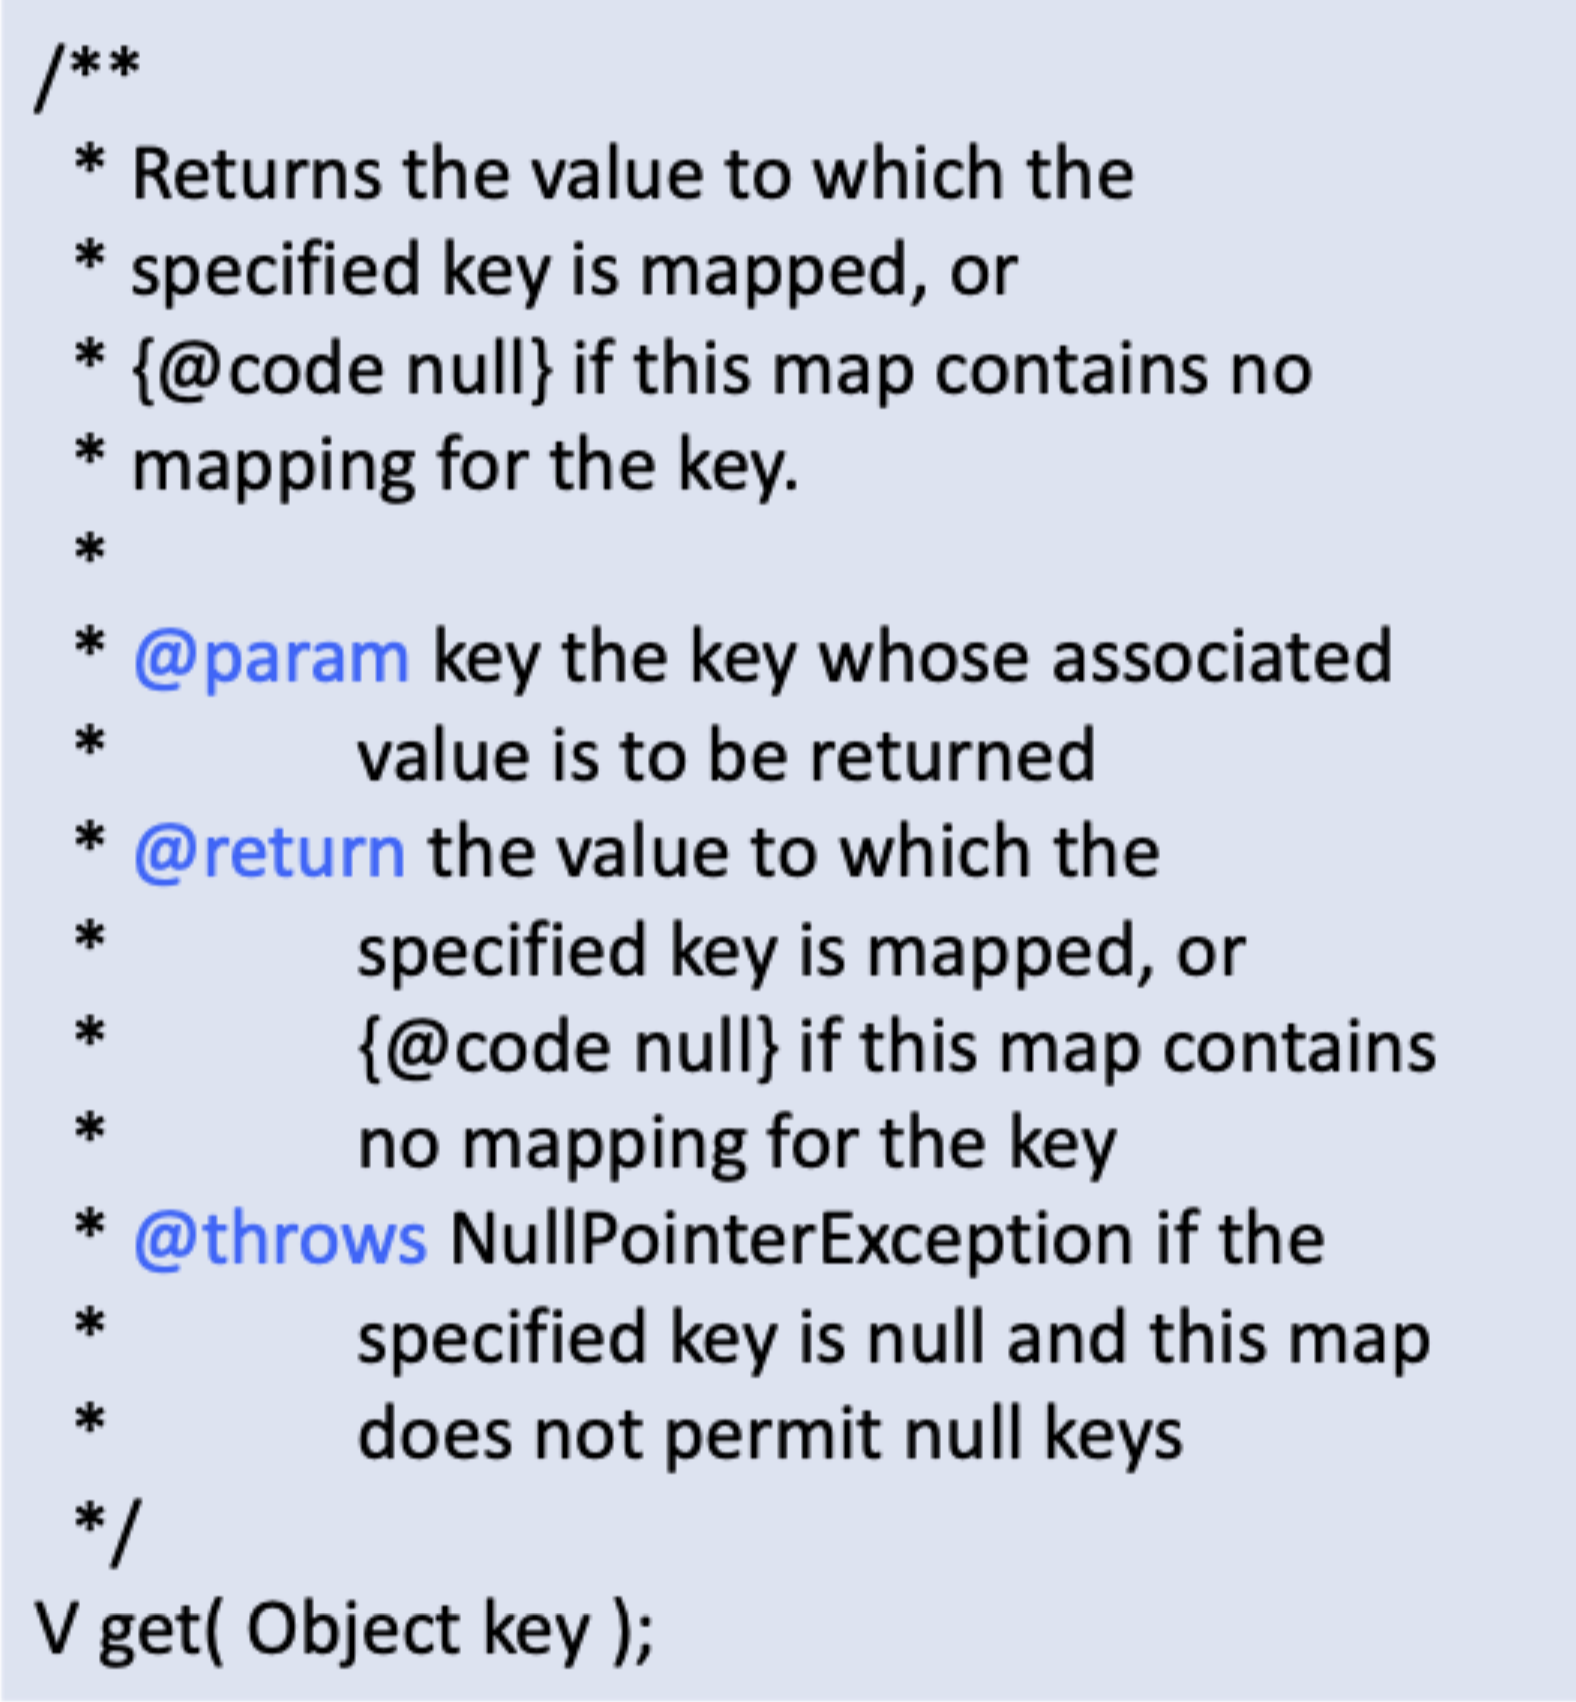
\includegraphics[width=0.5\columnwidth]{assets/comment}
\end{center}

Using diagrams and examples to illustrate complex concepts can help to make the documentation easier to understand. Using consistent formatting and naming conventions can further improve it. Finally, reviewing and updating the documentation regularly to ensure that it remains accurate and up-to-date.